\item \textbf{{[}YIJC/PRELIM/9569/2020/P2/Q4{]} }

\emph{SafeEnter} is a digital check-in system that tracks the people
visiting the public places, to prevent and control the transmission
of COVID-19 through contact tracing.
\begin{center}

\includegraphics[width=0.25\paperwidth]{C:/Users/Admin/Desktop/Github/question_bank/LyX/static/img/9569-YIJC-2020-P2-Q4-1}
\par\end{center}

\subsection*{Task 4.1}

Create a HTML file called \texttt{index.html} to display the Check-In
form for people to input their particulars and other details. (Use
the picture \texttt{IN.JPG} provided.) {[}5{]}
\begin{center}
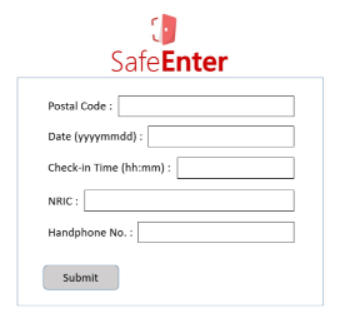
\includegraphics[width=0.25\paperwidth]{C:/Users/Admin/Desktop/Github/question_bank/LyX/static/img/9569-YIJC-2020-P2-Q4-2}
\par\end{center}

\noindent \begin{center}
Check-In Form
\par\end{center}

\subsection*{Task 4.2}

Write program code, \texttt{server.py}, for the back-end server to
display the Check-In form on the clients\textquoteright{} browser
when they scan a QR-code which links to the SafeEnter website. The
server script should include a route \textquoteleft \texttt{/checkin}\textquoteright{}
to receive the inputs from the client, the program code should: 
\begin{itemize}
\item prevent the user from accessing the \textquoteleft \texttt{/checkin}\textquoteright{}
route directly 
\item receive all the inputs in the Check-In form
\item reject empty or null inputs
\item append the new entry into the \texttt{event} table in the given database
\texttt{covid.db }
\item reply by sending a \texttt{checkout.html} page back to the client\textquoteright s
browser, displaying the following Check-Out form, which is to be used
when leaving the venue (Use the picture \texttt{OUT.JPG} provided.)\texttt{
}\hfill{}{[}12{]}
\end{itemize}
\begin{center}
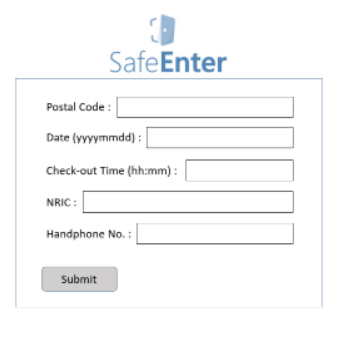
\includegraphics[width=0.25\paperwidth]{C:/Users/Admin/Desktop/Github/question_bank/LyX/static/img/9569-YIJC-2020-P2-Q4-3}
\par\end{center}

\noindent \begin{center}
Check-Out Form
\par\end{center}

\subsection*{Task 4.3}

Modify the program code, \texttt{server.py}, and include an additional
route \textquoteleft \texttt{/checkout}\textquoteright{} to receive
the inputs from the client\textquoteright s Check-Out form when they
leave the venue. The program code should: 
\begin{itemize}
\item allow the user from accessing the \textquoteleft /checkout\textquoteright{}
route directly 
\item receive all the inputs in the Check-Out form 
\item reject empty or null inputs 
\item update the corresponding entry in the \texttt{event} table in the
\textbf{given} database \texttt{covid.db }\hfill{}{[}8{]}
\end{itemize}
Download the files for your program codes for Task 4 as 

\texttt{Task4\_<your name>\_<centre number>\_<index number>\_index.html }

\texttt{Task4\_<your name>\_<centre number>\_<index number>\_checkout.html}

\texttt{Task4\_<your name>\_<centre number>\_<index number>\_server.py }

\texttt{Task4\_<your name>\_<centre number>\_<index number>\_covid.db}